\title{Study Guide for Final for Calculus-Based Physics-2: Electricity, Magnetism, and Thermodynamics (PHYS180-02)}
\author{Dr. Jordan Hanson - Whittier College Dept. of Physics and Astronomy}
\date{\today}
\documentclass[10pt]{article}
\usepackage[a4paper, total={18cm, 27cm}]{geometry}
\usepackage{outlines}
\usepackage[sfdefault]{FiraSans}
\usepackage{hyperref}
\usepackage{graphicx}
\begin{document}
\maketitle

\begin{enumerate}
\item \textbf{Temperature and Heat}
\begin{enumerate}
\item A metal bolt is manufactured slightly larger than the hole on a bulkhead in which it is to be inserted. The bolt is held at a different temperature when it is inserted. Should the bolt be hotter or colder than the bulkhead metal?
\begin{itemize}
\item A: Hotter
\item B: Colder
\item C: Same Temperature
\item D: It will not fit regardless of temperature
\end{itemize}
\item Recall that the linear expansion of materials is described by $\Delta L = \alpha L_0 \left(T_f - T_i \right)$.  The volumetric expansion coefficient of water is $\beta = 210 \times 10^{-6}$ C$^{\circ -1}$.  Calculate the height change in sea level due to a rise in water temperature of 2.0 C$^{\circ -1}$, for an an initial height of 5 km. \\ \vspace{2cm}
\end{enumerate}
\item \textbf{The Kinetic Theory of Gases}
\begin{enumerate}
\item How is momentum related to the pressure exerted by a gas? Explain on the molecular level, considering the behavior of molecules. \\ \vspace{1cm}
\item Recall that $pV = n R T$.  Suppose a small cylinder of fixed volume containing an ideal gas is subjected to temperature and pressure changes.  Which of the following is true?
\begin{itemize}
\item A: If the gas escapes such that the pressure drops but the moles are approximately constant, the tempreature will decrease.
\item B: If the gas escapes such that the pressure drops but the moles are approximately constant, the tempreature will increase.
\item C: If the gas escapes such that the pressure drops but the moles are approximately constant, the tempreature will remain constant.
\item D: None of the above.
\end{itemize}
\item Same cylinder of gas as prior question.  Which of the following is true?
\begin{itemize}
\item A: If the cylinder is cooled, the pressure will increase.
\item B: If the cylinder is cooled, the number of moles will decrease.
\item C: If the cylinder is cooled, the pressure will decrease.
\item D: None of the above.
\end{itemize}
\item If the pressure is 4 atm, and the volume is 0.5 L, and the temperature is $30.0$ C$^{\circ}$, how many moles of gas are in the cylinder?  ($R = 8.31$ J/mol/K).  If the temperature is changed to $20.0$ C$^{\circ}$, what is the new pressure? \\ \vspace{3cm}
\item Recall that $Q = n C_V \Delta T$, and that for an ideal monatomic gas, $C_V = \frac{3}{2}R$.  How much heat is required to raise the temperature of the gas by $10$ C$^{\circ}$?  How does this answer change if the gas is diatomic, and all degrees of freedom must be taken into account? \\ \vspace{3cm}
\end{enumerate}
\item \textbf{The First Law of Thermodynamics}
\begin{enumerate}
\item Recall that $\Delta E_{int} = Q - W$.  Which of the following is true?
\begin{itemize}
\item A: For isothermal processes, $Q = W$.
\item B: For isochoric processes, $\Delta E_{int} = Q$.
\item C: For adiabatic processes, $\Delta E_{int} = -W$.
\item D: All of the above.
\end{itemize}
\item Recall that $\Delta E_{int} = Q - W$.  Suppose a machinist is polishing a copper fitting.  Which of the following is true, if all of the work done on the copper contributes to the rise in temperature of the copper?
\begin{itemize}
\item A: The copper loses some heat to the environment.
\item B: The copper does work on the machinist.
\item C: The copper loses some heat to the environment.
\item D: The copper does work on the environment.
\end{itemize}
\item Recall that $Q = n C_P \Delta T$, and that for an ideal monatomic gas, $C_P = C_V + R$.  What is the heat required to raise the temperature of 10 moles of diatomic ideal gas at constant \textit{pressure}?  At constant \textit{volume}? \\ \vspace{3cm}
\end{enumerate}
\item \textbf{The Second Law of Thermodynamics}
\begin{enumerate}
\item Recall that the efficiency of a Carnot style engine is $e = 1-\frac{T_c}{T_h}$.  Suppose an engine is run at $T_h = 1500$ K, and $T_c = 500$ K.  What is the efficiency?  If the heat required to run the engine ($Q_h$) is 2 kJ, what is the work done by the engine per cycle?  \\ \vspace{3cm}
\end{enumerate}
\item \textbf{Electric Charges and Fields}
\begin{enumerate}
\item Recall that $\vec{F} = k \frac{q_1 q_2}{r^2}\hat{r}$.  Four charges are all on the x-axis, with equal distances between them.  At what locations, if any, is the force equal to zero?  What happens to a positive test charge placed halfway between the middle two charges?  What happens when the test charge is placed halfway between one of the outer charges and the outer charge's neighbor? \\ \vspace{4cm}
\item Recall that $\vec{E} = k \frac{q_1}{r^2}\hat{r}$.  Draw the electric field of 1) a point charge 2) an electric dipole (two charges separated by some distance and of opposite magnitude).  Add equipontial lines, or lines indicating common electric potential (voltage). \\ \vspace{5cm}
\item Which of the following is true of an infinite line of charge oriented along the z-axis?
\begin{itemize}
\item A: The field increases with increasing distance from the line charge.
\item B: The field decreases with increasing distance from the line charge.
\item C: The field does not depend on $x$ or $y$.
\item D: The field has a $\hat{z}$ component.
\item E: B and C
\end{itemize}
\item Which of the following is true of an infinite plane of charge oriented in the $x-y$ plane?
\begin{itemize}
\item A: The field does not depend on $x$ or $y$.
\item B: The field decreases with increasing $z$.
\item C: The field does not depend on $z$.
\item D: The field decreases with increasing $x$ and $y$.
\item E: A and C.
\end{itemize}
\end{enumerate}
\item \textbf{Gauss's Law}
\begin{enumerate}
\item Suppose an infinite plate of charges is oriented in the $x-y$ plane, and the charge per unit surface area is $\sigma$.  Using Gauss' Law, show or explain how the electric field is $\vec{E} = \sigma/\epsilon_0 \hat{z}$. \\ \vspace{3cm}
\item If the charge density is $10$ nC per mm$^2$, and $\epsilon_0 = 8.85 \times 10^{-12}$ N$^{-1}$ m$^{-2}$ C$^2$, what is the value of the electric field?  Will this field change if the plate of charge is rotated?  \\ \vspace{2cm}
\end{enumerate}
\item \textbf{Electric Potential}
\begin{enumerate}
\item Suppose two plates identical to the one in the previous problem are both parallel to the $x-y$ plane, and separated by a distance $z_0$.  If the charge densities are equal and opposite, the voltage associated with the electric field between the plates is
\begin{itemize}
\item A: A quadratic function of $z$.
\item B: A cubic function of $z$.
\item C: A linear function of $z$.
\item D: Constant
\item E: B and C
\end{itemize}
\item If the voltage difference between the plates is 100 V, what is the separation $z_0$? \\ \vspace{2cm}
\item What is the electric field associated with the voltage $V(x,y,z) = V_0 \left( x^2 + y^2 \right)$?  Remember to express your answer as a \textit{vector field}, not just a magnitude of a field.  \\ \vspace{2cm}
\end{enumerate}
\item \textbf{Current and Resistance}
\begin{enumerate}
\item Recall that $V = iR$, and that $R = \frac{\rho L}{A}$.  Suppose current is flowing through a cylindrical conductor with radius $r$ and length $l$.  The voltage driving the current remains constant.  Choose all that are true:
\begin{itemize}
\item A: Increasing $r$ decreases the current.
\item B: Decreasing $l$ decreases the current.
\item C: Decreasing $l$ increases the current.
\item D: Increasing $r$ increases the current.
\end{itemize}
\begin{figure}[hb]
\centering
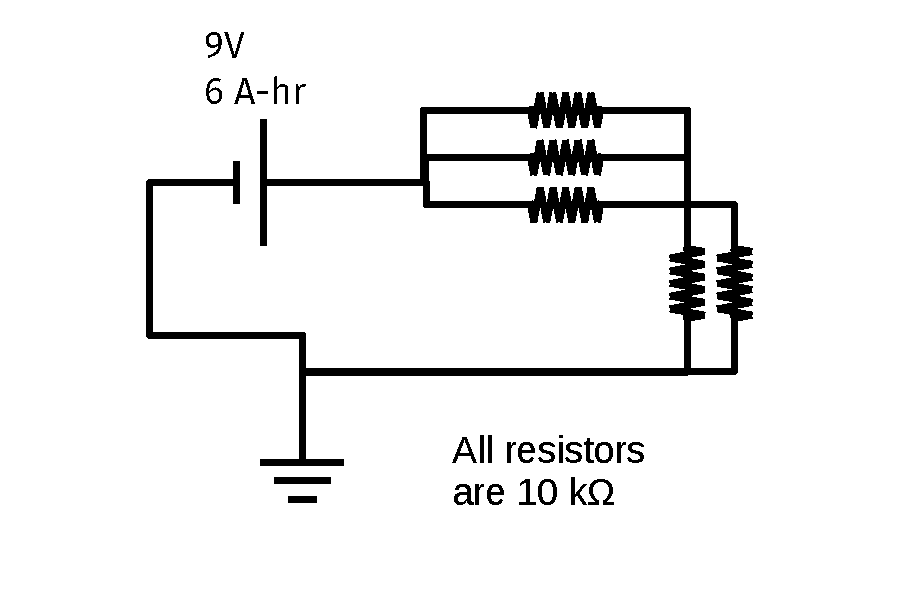
\includegraphics[width=0.5\textwidth]{figures/circuitExample1.pdf}
\caption{\label{fig:circuit} A DC circuit with a battery voltage of 9V and five identical resistors.}
\end{figure}
\item Consider the circuit in Fig. \ref{fig:circuit}.  How long before the battery runs out? \\ \vspace{3cm}
\end{enumerate}
\item \textbf{Magnetic Forces and Fields}
\begin{enumerate}
\begin{figure}
\centering
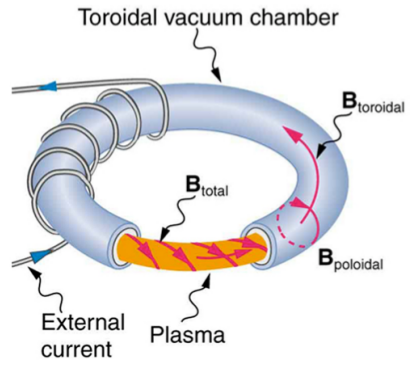
\includegraphics[width=0.45\textwidth]{figures/tok.png}
\caption{\label{fig:tok} The basic premise of a tokamak, containing plasma for fusion reactions.}
\end{figure}
\item \textit{Recall that $\vec{F} = q\vec{v} \times \vec{B}$.} The toroidal magnetic field in the tokamak fusion reactor in Fig. \ref{fig:tok} is created by the external current.  The plasma is hot ionized gas, and the \textit{poloidal} magnetic field is created by it.  In which direction is the plasma flowing, and which law of physics creates the poloidal field as a result?
\begin{itemize}
\item A: Counter-clockwise, Faraday's Law
\item B: Counter-clockwise, Amp\`{e}re's Law
\item C: Clockwise, Faraday's Law
\item D: Clockwise, Amp\`{e}re's Law
\end{itemize}
\item Suppose in a region of the tokamak the toroidal field is $\vec{B} = B_0 \hat{y}$.  If a positively charged particle has a velocity $\vec{v} = v_0 \vec{z}$, in which direction is it accelerated?
\end{enumerate}
\end{enumerate}
\end{document}